\section{Sprint 2 Summary}

At the end of sprint 1, the group had decided on a concept for the flight controller. Our plan was to use the motion capture system Qualisys at KIC as our only source of sensing and do all computations externally. The concept was to have no on-board computation, only a receiver on the quadcopter and a unit to send PWM-signals to the motors. In this way, we could eliminate the need for a on-board chip. 
\\
Week one of sprint 2, was our first week of technical work. The first thing we did, was to investigate if it was possible to use Qualisys as our control system. To investigate if it was possible, the group transferred data between Qualisys and an Arduino, and measured the time taken. Additionally, the group built a test rig to see if we could hold a motor-propeller assembly on closed-loop control from Qualisys to see if it was possible to achieve stability.


\begin{figure}[h]
        \centering
        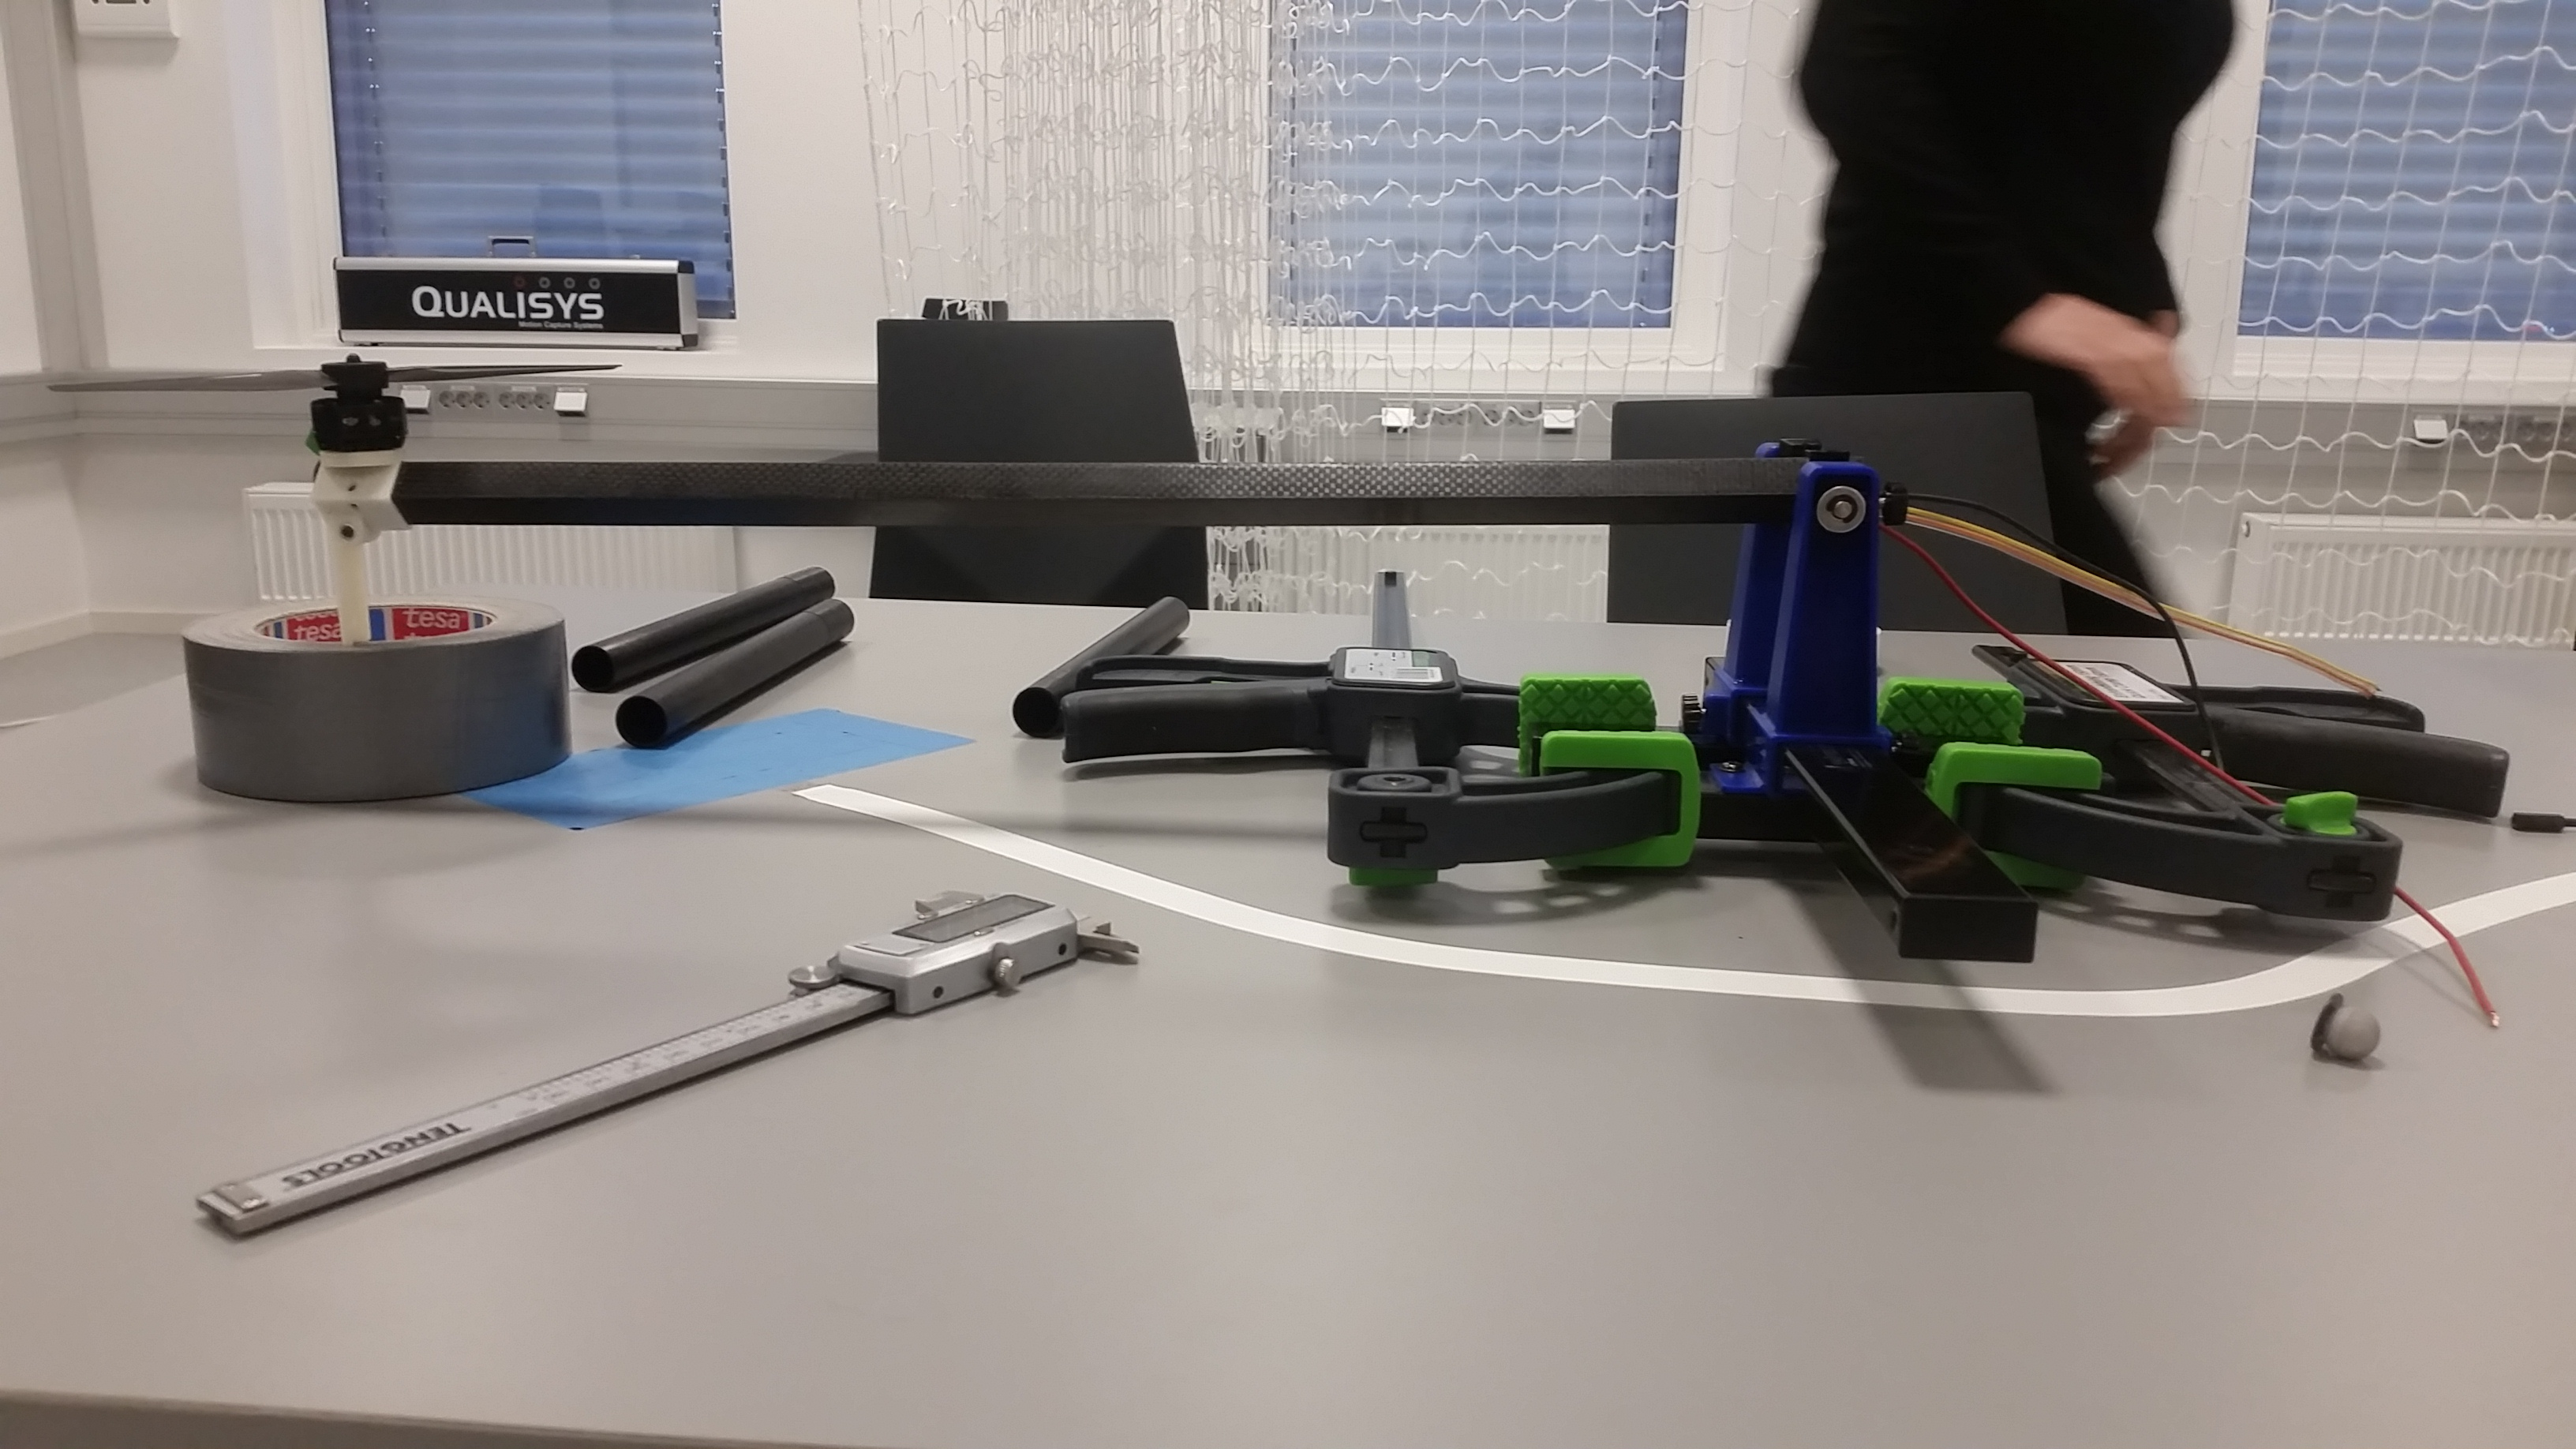
\includegraphics[width = 0.5
        \textwidth]{VAPIQ-PICTURES//TestRig(arm)1}
         \caption{First Test Rig}
        %\\[2.0 cm]
       
    \end{figure}   
\noindent
The group then quickly realised that the latency in Qualisys was to great, and concluded that it would be impossible to achieve stable flight with the motion capture system by itself, without on-board computation.
\\
In this sprint, construction of the fixed pitch quadcopter was postponed. The original plan was to use motors which could handle both variable and fixed pitch, in this way we could build two similar quadcopters which could be compared as equal. Since the motors and mechanisms the group ordered did not work, a new plan and new orders had to be placed. 
\\
In the meantime, a simple laser-cut fixed pitch quadcopter was assembled with motors lent from HSN to test our control algorithm. This was a rapid prototype and only meant for the test bench. In this sprint the preliminary web-page was also published.

\begin{figure}[h]
        \centering
        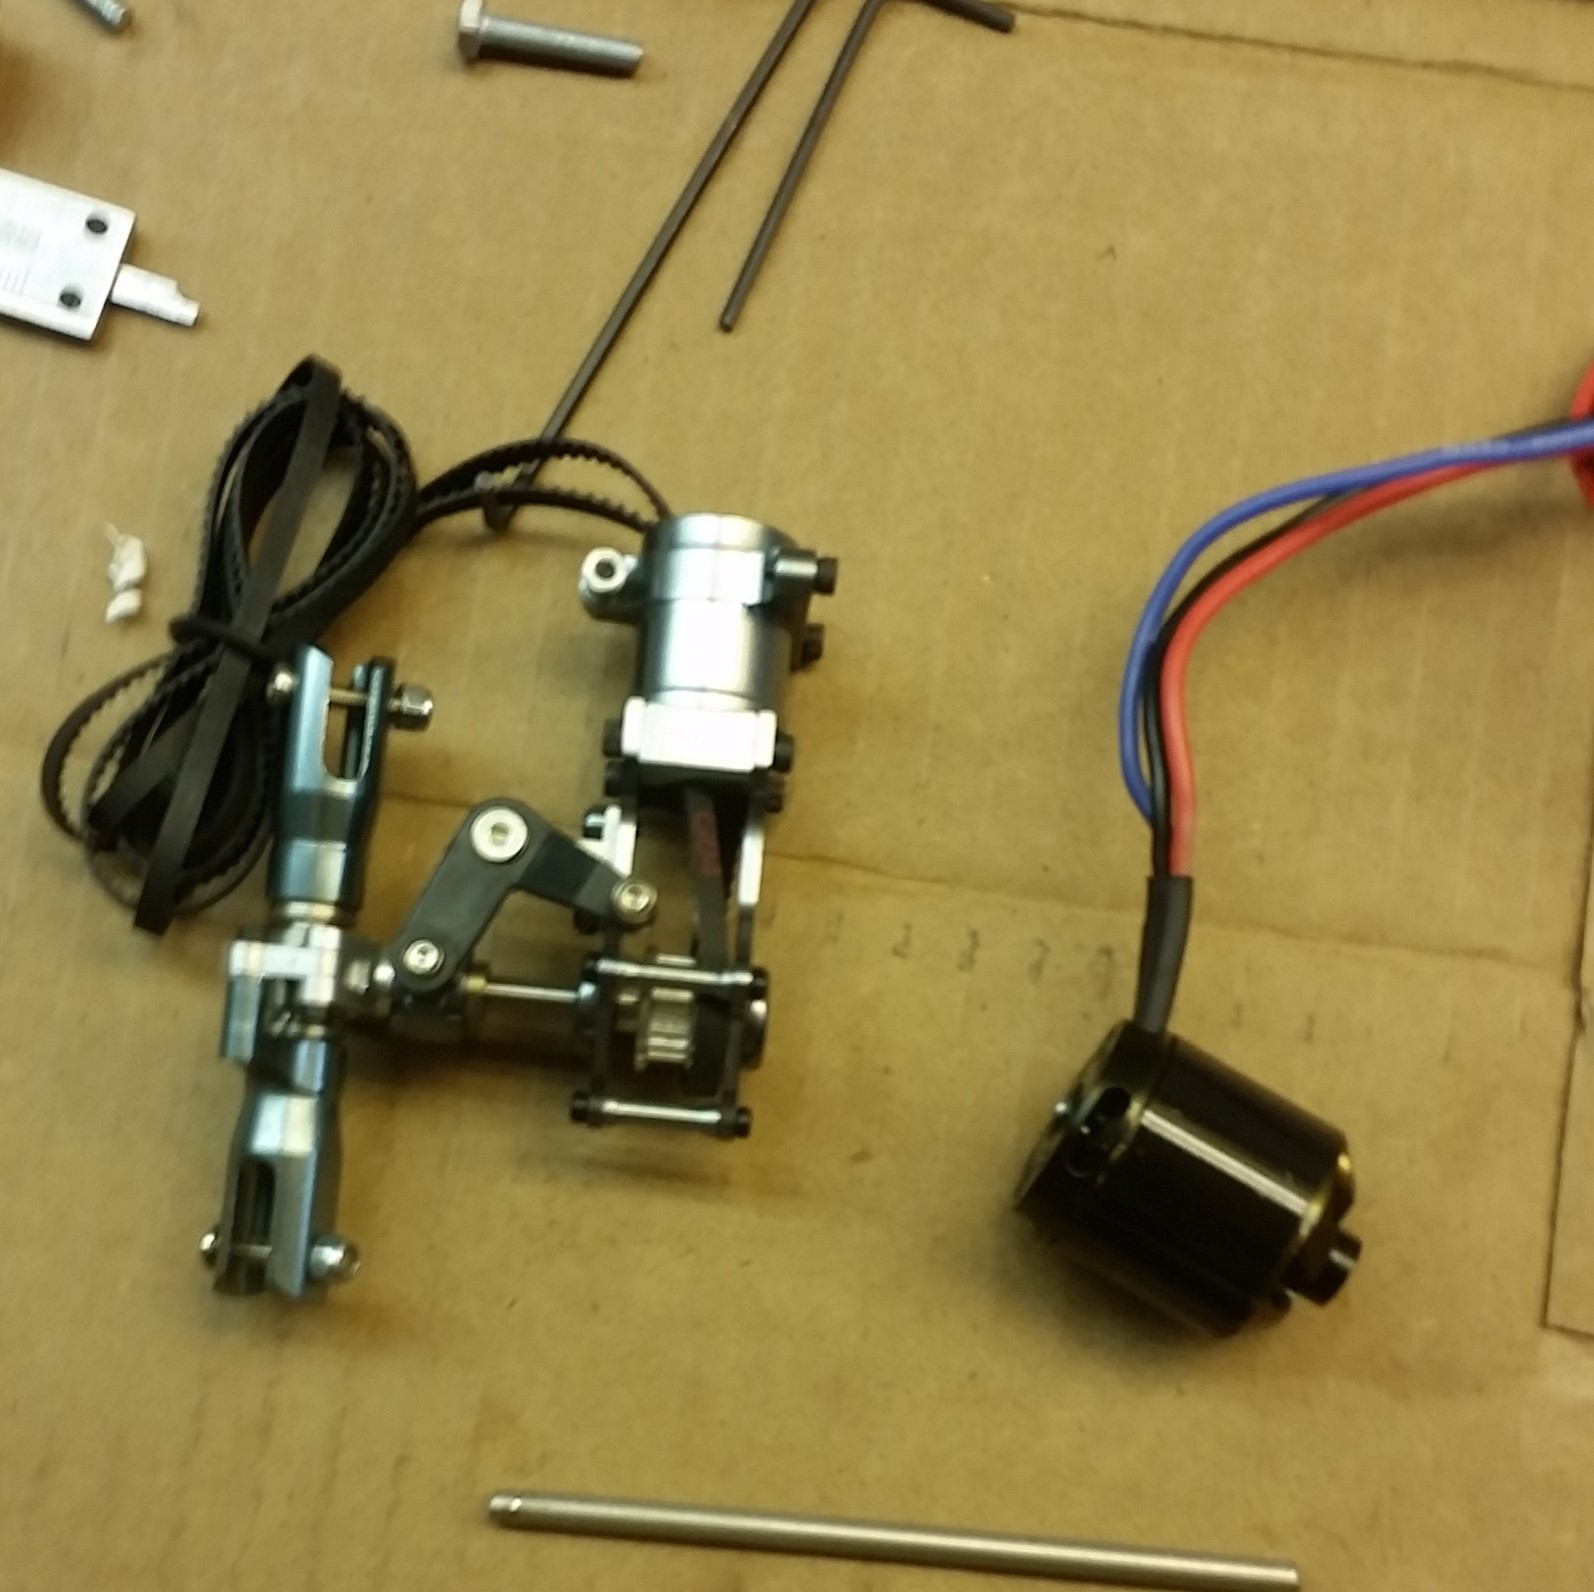
\includegraphics[width = 0,8
        \textwidth]{VAPIQ-PICTURES//BeforeAssembly.jpg}
         \caption{First Fixed Pitch Test Copter}
        %\\[2.0 cm]
    \end{figure}  

\begin{comment}
 - Webpage release
 - Fear of ordering more wrong parts.
 -
 -
\end{comment}
\newpage
        

\subsection{Completion and Scope Change, Sprint 2}


In sprint 2, 79\% of work was completed and the scoop change was 35\%. The scope change was mainly due to the fact that our original plan of using Qualisys as the control system did not work. Therefore we had to reevaluate and find another solution. The group also had plans of making the first fixed pitch quadcopter, but the motors we planned to use were destroyed. 
\\
Because of the changes in scope, some activities in the project plan had to be postponed to sprint 3.
\\\\
Project plan status, sprint 2:

\begin{itemize}
    \item 	Electrical Analysis, \textbf{Postponed}
    \item   Electrical Layout, \textbf{Postponed}
    \item   Electrical Construction, \textbf{Postponed}
    \item   Mathematical Model, Fixed Pitch, \textbf{Postponed}
    \item 	Bluetooth Communication With Arduino, \textbf {Postponed}
    \item 	Mechanical Design Plan, Fixed Pitch, \textbf{Started}
    \item 	Prototype, Fixed Pitch, \textbf{Postponed} (only made a simple test copter)
   	\item   Flight Controller Software, \textbf{Started}
    \item 	Publish Web Page, \textbf{Done}
\end{itemize}

\begin{figure}[h]
        \centering
        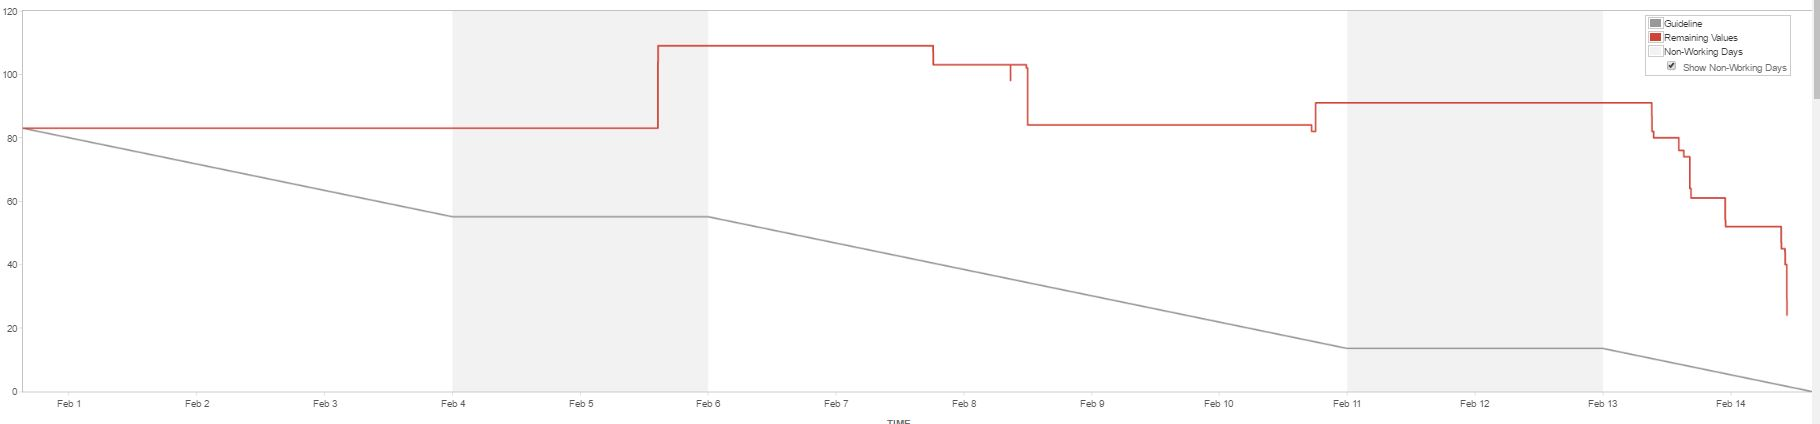
\includegraphics[width = 1
        \textwidth]{VAPIQ-PICTURES//SprintBD2}
         \caption{Burndown Chart Sprint 2}
        %\\[2.0 cm]
       
    \end{figure}    

\subsection{Challenges}

The original mechanisms the group got and the plan to use Qualisys to control the quadcopter did not work, so we had to come up with a new solution. We also had problems with bluetooth communication because of defect electronics, but have since been resolved.

\subsection{Lessons Learned}

Be sceptical of Chinese hardware bought online. Make sure that the computation takes no more than 20 ms.  

